\section{Simulation Analysis}
\label{sec:simulation}

\subsection{Operating Point Analysis}

Table~\ref{tab:p1} shows the simulated operating point results for the circuit
under analysis. When compared to the theoretical analysis results, we see the same values
up to the 5 decimal places provided by ngspice.

\begin{table}[H]
  \centering
  \begin{tabular}{|l|r|}
    \hline    
    {\bf Name} & {\bf Value [A or V]} \\ \hline
    @ca[i] & 0.000000e+00\\ \hline
@gb[i] & -2.53212e-04\\ \hline
@r1[i] & 2.414774e-04\\ \hline
@r2[i] & 2.532123e-04\\ \hline
@r3[i] & -1.17349e-05\\ \hline
@r4[i] & -1.20106e-03\\ \hline
@r5[i] & -2.53212e-04\\ \hline
@r6[i] & 9.595831e-04\\ \hline
@r7[i] & 9.595831e-04\\ \hline
v(1) & 5.136122e+00\\ \hline
v(2) & 4.884647e+00\\ \hline
v(3) & 4.361951e+00\\ \hline
v(5) & 4.920010e+00\\ \hline
v(6) & 5.690271e+00\\ \hline
v(8) & -2.94454e+00\\ \hline
v(71) & -1.96654e+00\\ \hline
v(72) & -1.96654e+00\\ \hline

  \end{tabular}
  \caption{Operating point. A variable preceded by @ is of type {\em current}
    and expressed in Ampere; other variables are of type {\it voltage} and expressed in
    Volt.}
  \label{tab:p1}
\end{table}

\begin{table}[H]
    \centering
    \begin{tabular}{|l|r|}
      \hline    
      {\bf Name} & {\bf Value [A or V]} \\ \hline
      @gb[i] & -6.24390e-18\\ \hline
@r1[i] & 5.954528e-18\\ \hline
@r2[i] & 6.243896e-18\\ \hline
@r3[i] & -2.89368e-19\\ \hline
@r4[i] & 1.300919e-18\\ \hline
@r5[i] & -2.83857e-03\\ \hline
@r6[i] & -8.67362e-19\\ \hline
@r7[i] & 1.165891e-21\\ \hline
v(1) & 0.000000e+00\\ \hline
v(2) & -6.20107e-15\\ \hline
v(3) & -1.90901e-14\\ \hline
v(5) & -5.32907e-15\\ \hline
v(6) & 8.634810e+00\\ \hline
v(8) & 1.776357e-15\\ \hline
v(71) & 1.777545e-15\\ \hline
v(72) & 1.777545e-15\\ \hline

    \end{tabular}
    \caption{Operating point. A variable preceded by @ is of type {\em current}
      and expressed in Ampere; other variables are of type {\it voltage} and expressed in
      Volt.}
    \label{tab:p2}
  \end{table}

\subsection{Natural response}

  \begin{figure}[H] \centering
    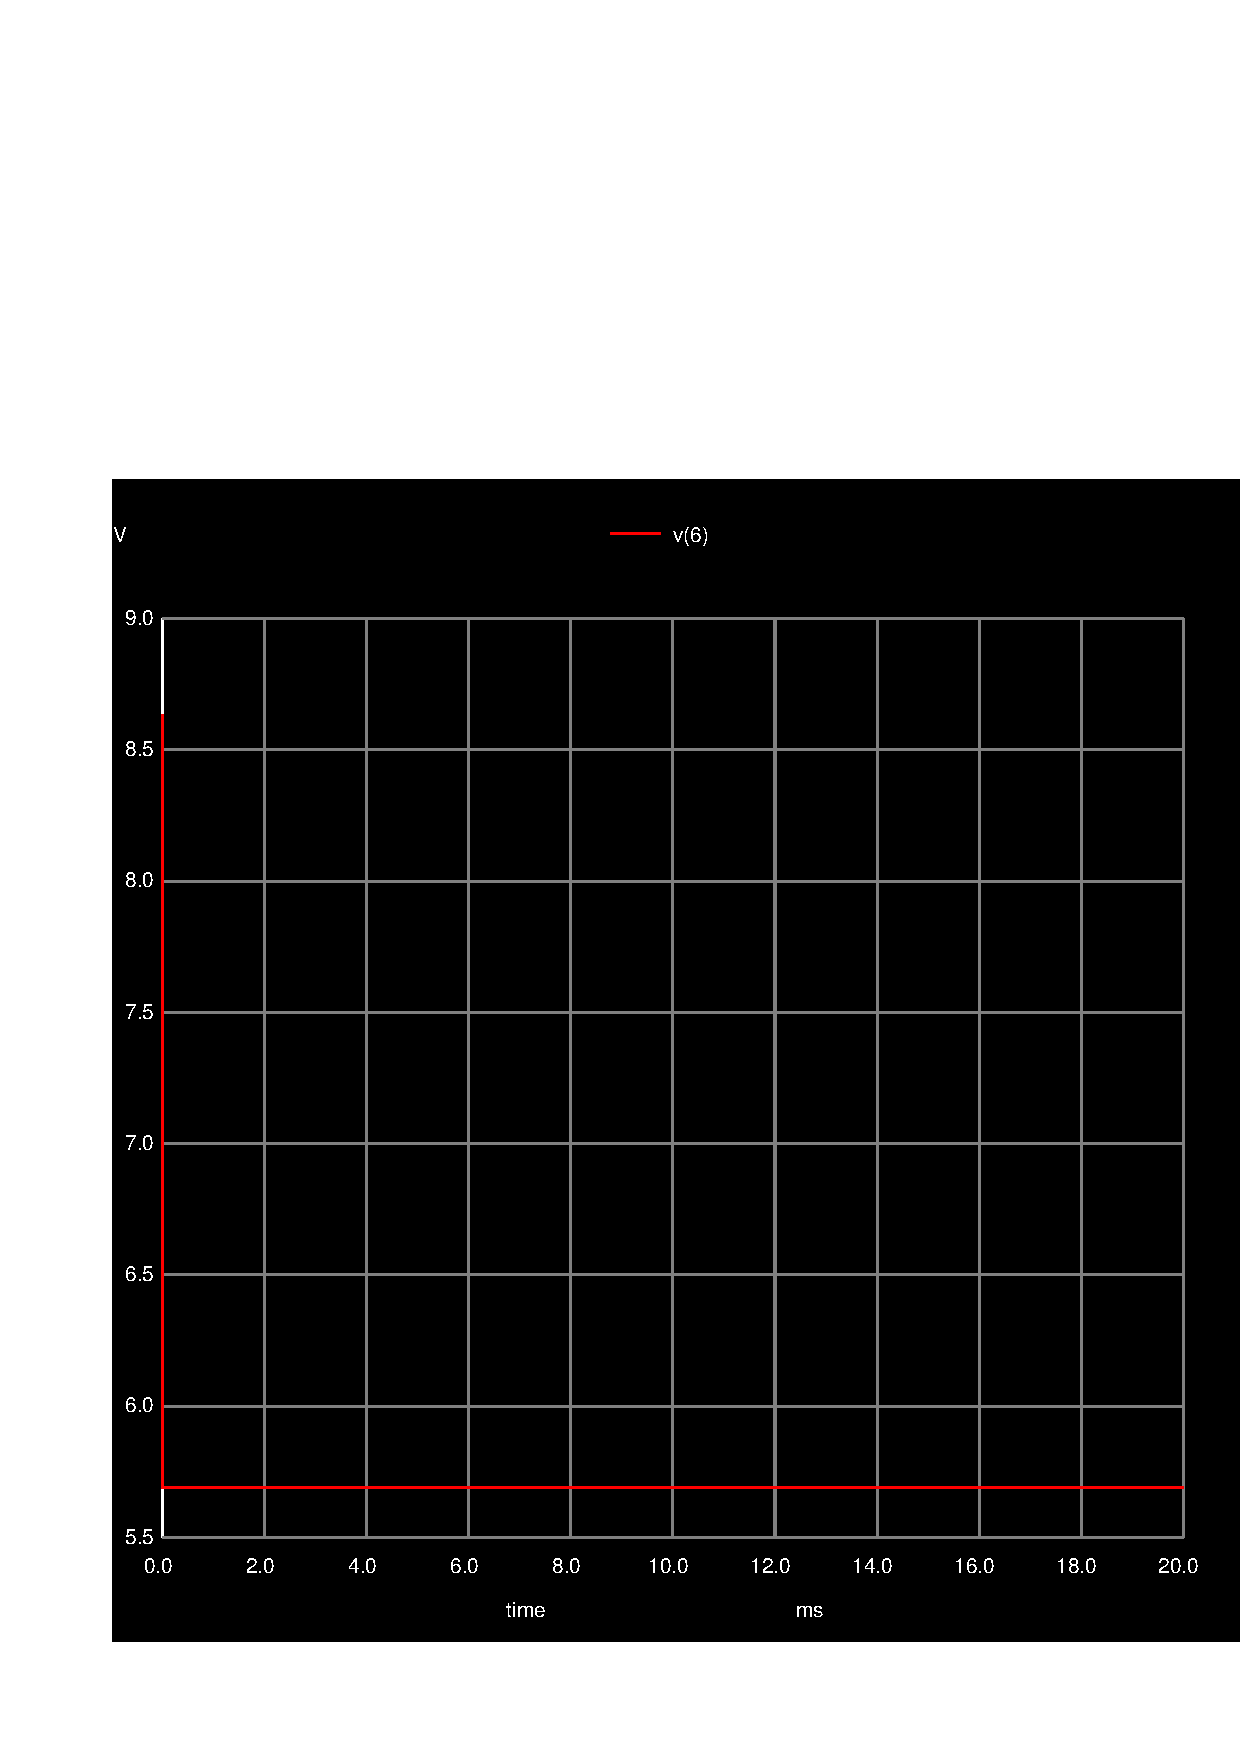
\includegraphics[width=1\linewidth]{../sim/trans3.pdf}
    \caption{RC circuit to be analysed}
    \label{fig:t2}
    \end{figure}

  \subsection{Forced response}


  \begin{figure}[H] \centering
    \includegraphics[width=1\linewidth]{../sim/trans4.pdf}
    \caption{RC circuit to be analysed}
    \label{fig:t2}
    \end{figure}

  \subsection{Frequency analysis}

  \begin{figure}[H] \centering
    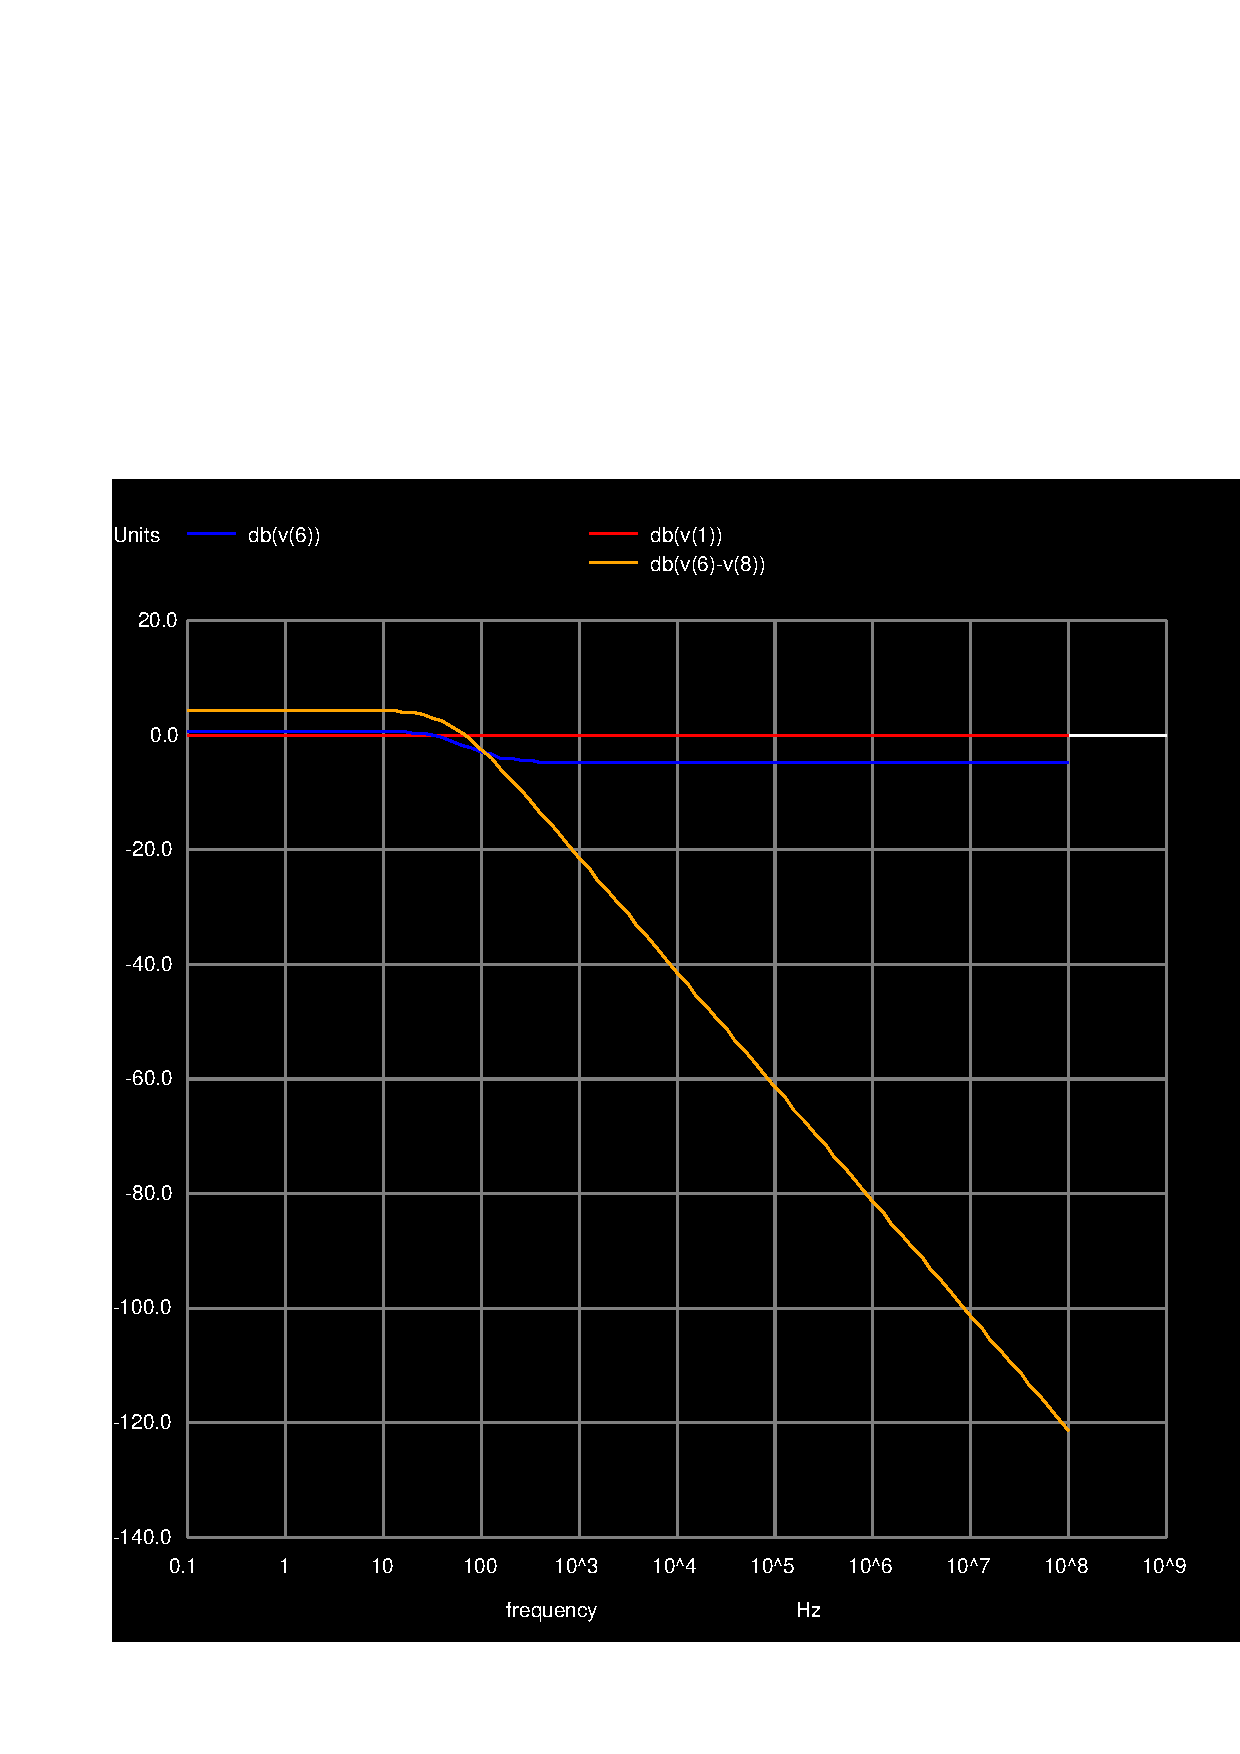
\includegraphics[width=1\linewidth]{../sim/mag5.pdf}
    \caption{RC circuit to be analysed}
    \label{fig:t2}
    \end{figure}

    \begin{figure}[H] \centering
        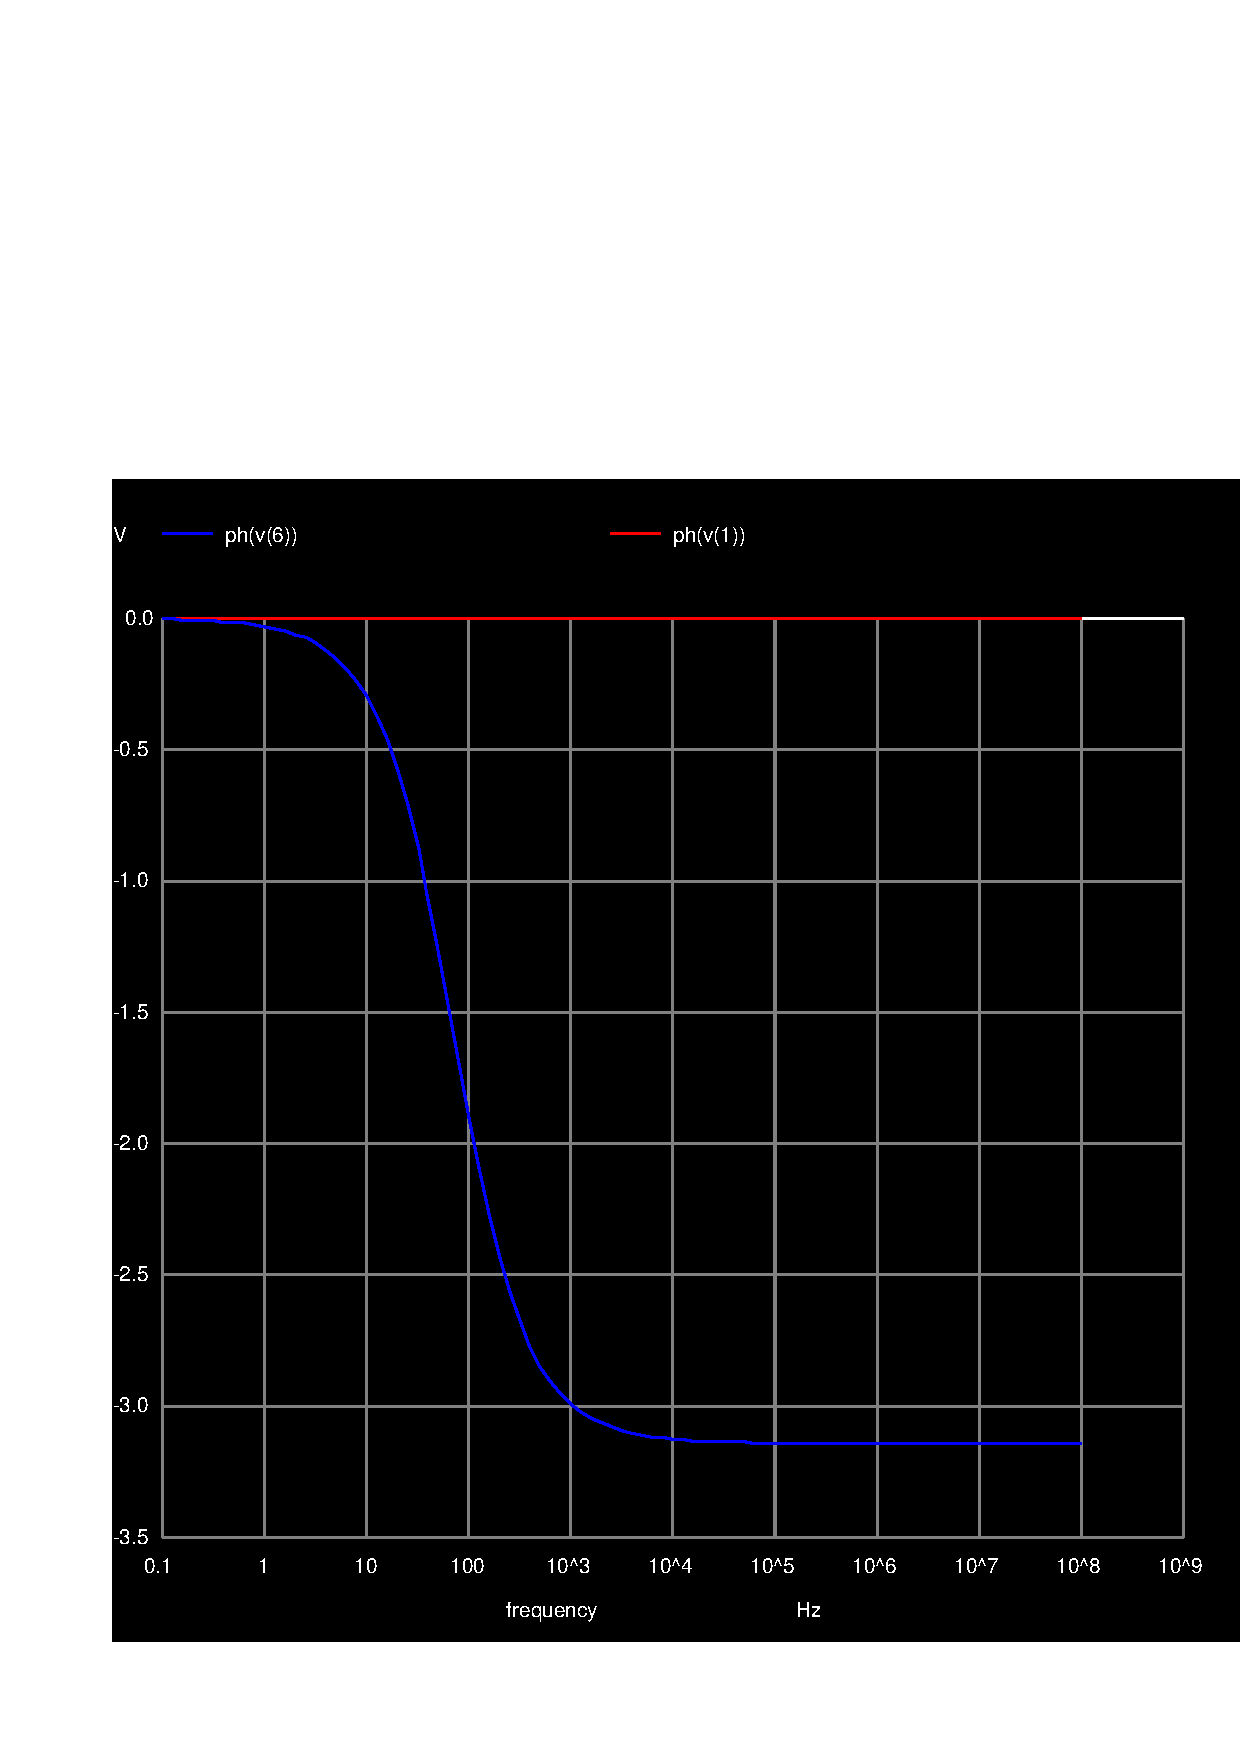
\includegraphics[width=1\linewidth]{../sim/phase5.pdf}
        \caption{RC circuit to be analysed}
        \label{fig:t2}
        \end{figure}

It should be noted that nodes G1 and G2 represent the same node G, and exist seperatly
so as to allow the measuring of current $I_c$ in ngspice, for the purpose of defining the
dependent voltage source $V_c$.

